\fancyhead[L]{\textsf{\textbf{54}}\quad \textbf{\textsf{CHƯƠNG 1}}\quad \textsf{Hàm số và Mô hình}}
\fancyhead[R]{}
\noindent
\begin{minipage}[t]{0.26\textwidth}
    \vspace{0pt}
    % 5 đường kẻ trang trí ở đầu trang đối xứng với mục 1.5
    \vspace*{6pt}
    \noindent{\color{stewartcyan}%
    \rule{\linewidth}{0.6pt}\\[2.5pt]
    \rule{\linewidth}{0.6pt}\\[2.5pt]
    \rule{\linewidth}{0.6pt}\\[2.5pt]
    \rule{\linewidth}{0.6pt}\\[2.5pt]
    \rule{\linewidth}{0.6pt}}

    % Khoảng cách dóng Hình 1 ngang hàng với Bảng 1 & 2
    \vspace{182pt}
    \begin{center}
        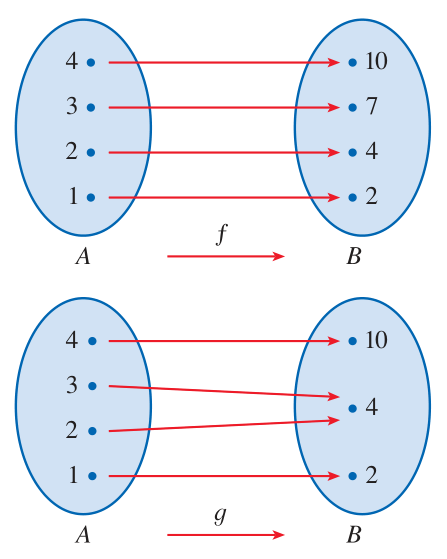
\includegraphics[width=0.95\linewidth]{images/p0089_fig1.png}
    \end{center}
    \vspace{-6pt}
    \noindent\textbf{\textsf{HÌNH 1}}\\[2pt]
    {\small $f$ là hàm một-đối-một; $g$ thì không.}
    
    \vspace{1.5em}
    \noindent{\small Dưới góc độ đầu vào và đầu ra, Định nghĩa~1 phát biểu rằng $f$ là hàm một-đối-một nếu mỗi đầu ra chỉ tương ứng với duy nhất một đầu vào.}

    \vspace{1.5em}
    \begin{center}
        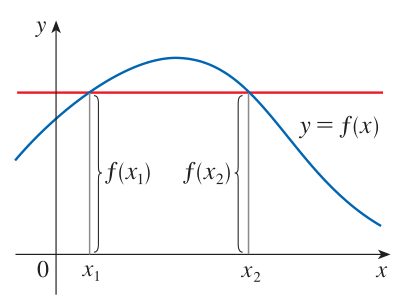
\includegraphics[width=\linewidth]{images/p0089_fig2.png}
    \end{center}
    \vspace{-6pt}
    \noindent\textbf{\textsf{HÌNH 2}}\\[2pt]
    {\small Hàm số này không phải là hàm một-đối-một vì $f(x_1) = f(x_2)$.}
\end{minipage}%
\hfill
\begin{minipage}[t]{0.71\textwidth}
    \vspace{0pt}
    \noindent{\Huge\color{stewartcyan}\textbf{\textsf{1.5}}}\;\;% nội dung tiêu đề có vạch đứng
    {\color{stewartcyan}\rule[-4pt]{1.5pt}{24pt}}\;\;% 
    {\LARGE\textbf{\textsf{Hàm số ngược và Hàm số Lôgarit}}}
    \vspace{0.8em}

    \noindent{\color{stewartcyan}\rule{6.5pt}{6.5pt}}\;\; \textbf{\large\textsf{Hàm số ngược}}

    \vspace{0.41em}
    \noindent Bảng 1 cung cấp dữ liệu từ một thí nghiệm trong đó nhà sinh học bắt đầu nuôi cấy vi khuẩn với 100 cá thể ban đầu trong môi trường dinh dưỡng giới hạn; kích thước của quần thể vi khuẩn được ghi lại theo từng khoảng thời gian mỗi giờ. Số lượng vi khuẩn $N$ là một hàm số theo thời gian $t$: $N = f(t)$.

    Tuy nhiên, giả sử nhà sinh học thay đổi góc nhìn và quan tâm đến thời gian cần thiết để quần thể đạt đến các mức số lượng khác nhau. Nói cách khác, bà ấy đang coi $t$ là một hàm số theo $N$. Hàm số này được gọi là \emph{hàm số ngược} của $f$, ký hiệu là $f^{-1}$, và đọc là ``$f$ ngược''. Ở đây $t = f^{-1}(N)$ là thời gian cần thiết để quần thể đạt đến mức $N$. Các giá trị của $f^{-1}$ có thể tìm được bằng cách đọc Bảng 1 từ phải sang trái hoặc bằng cách tra cứu Bảng 2. Chẳng hạn, $f^{-1}(550) = 6$ vì $f(6) = 550$.

    \vspace{0.66em}
    \begin{center}
        \small
        \begin{tabular}{cc}
            \textbf{\textsf{BẢNG 1}} \enspace $N$ là hàm theo $t$ & \textbf{\textsf{BẢNG 2}} \enspace $t$ là hàm theo $N$ \\[4pt]
            \begin{tabular}{|c|c|}
                \hline
                $t$ (giờ) & \makecell{$N = f(t)$\\ = số lượng tại thời điểm $t$} \\
                \hline
                0 & 100 \\
                1 & 168 \\
                2 & 259 \\
                3 & 358 \\
                4 & 445 \\
                5 & 509 \\
                6 & 550 \\
                7 & 573 \\
                8 & 586 \\
                \hline
            \end{tabular}
            &
            \begin{tabular}{|c|c|}
                \hline
                $N$ & \makecell{$t = f^{-1}(N)$\\ = thời gian đạt $N$ vi khuẩn} \\
                \hline
                100 & 0 \\
                168 & 1 \\
                259 & 2 \\
                358 & 3 \\
                445 & 4 \\
                509 & 5 \\
                550 & 6 \\
                573 & 7 \\
                586 & 8 \\
                \hline
            \end{tabular}
        \end{tabular}
    \end{center}

    \vspace{0.41em}
    \noindent Không phải mọi hàm số đều có hàm ngược. Hãy so sánh các hàm $f$ và $g$ có sơ đồ mũi tên được thể hiện trong Hình 1. Chú ý rằng $f$ không bao giờ nhận cùng một giá trị hai lần (hai đầu vào bất kỳ trong $A$ đều có các đầu ra khác nhau), trong khi $g$ lại nhận cùng một giá trị hai lần (cả 2 và 3 đều cho cùng giá trị đầu ra là 4). Dưới dạng ký hiệu,
    \[
        g(2) = g(3)
    \]
    \vspace{-1.2em}
    \noindent nhưng \hfill $f(x_1) \neq f(x_2) \quad \text{mỗi khi } x_1 \neq x_2$ \hfill\null
    \vspace{0.6em}

    \noindent Các hàm số có cùng tính chất này với $f$ được gọi là \emph{hàm một-đối-một} (hay \emph{hàm đơn ánh}).

    \vspace{0.66em}
    \begin{tcolorbox}[colback=white, colframe=stewartred, arc=0mm, boxrule=0.8pt, left=8pt, right=8pt, top=6pt, bottom=6pt]
        \noindent\colorbox{stewartred}{\textcolor{white}{\textbf{\textsf{1}}}}\; \textbf{\textsf{\color{stewartred}Định nghĩa}}\quad Một hàm số $f$ được gọi là \textbf{hàm một-đối-một} (hay \textbf{đơn ánh}) nếu nó không bao giờ nhận cùng một giá trị hai lần; nghĩa là,
        \[
            f(x_1) \neq f(x_2) \quad \text{mỗi khi } x_1 \neq x_2
        \]
    \end{tcolorbox}

    \vspace{0.66em}
    \noindent Nếu một đường thẳng nằm ngang cắt đồ thị của hàm số $f$ tại nhiều hơn một điểm, thì từ Hình 2 ta thấy tồn tại các số $x_1$ và $x_2$ sao cho $f(x_1) = f(x_2)$. Điều này có nghĩa là $f$ không phải là hàm một-đối-một.

    Do đó, ta có phương pháp hình học sau đây để xác định xem một hàm số có phải là hàm một-đối-một hay không.

    \vspace{0.66em}
    \begin{tcolorbox}[colback=white, colframe=stewartred, arc=0mm, boxrule=0.8pt, left=8pt, right=8pt, top=6pt, bottom=6pt]
        \textbf{\textsf{\color{stewartred}Kiểm định đường nằm ngang}}\quad Một hàm số là một-đối-một khi và chỉ khi không có đường thẳng nằm ngang nào cắt đồ thị của nó nhiều hơn một lần.
    \end{tcolorbox}
\end{minipage}